%% applications, benchmarks
%% jobs == instance of an application

\section{Evaluation}
In this section we evaluate \SYSTEM{}. We first describe our
experimental setup, then evaluate the \SYSTEM{}-based schedulers, and
finally present statistical analysis on \SYSTEM{} prediction accuracy
and overhead.

\subsection{Experimental Setup}
\label{sec:setup}

\subsubsection{Experimental System and Benchmarks}
Our test platform is composed of four dual-socket Ubuntu 14.04 system
with SuperMICRO X9DRL-iF motherboards and two Intel Xeon E5-2690
processors.  These processors have eight cores, hyper-threading (eight
additional virtual cores), and TurboBoost.  Each node has 64 GB of
RAM.

We use 15 benchmarks from different suites including PARSEC
(\texttt{blackscholes}, \texttt{fluidanimate}, \texttt{swaptions},
\texttt{x264}) \cite{parsec}, Minebench (\texttt{Kmeans},
\texttt{HOP}, \texttt{svmrfe}) \cite{minebench}, Rodinia
(\texttt{cfd}, \texttt{particlefilter}, \texttt{vips}, \texttt{btree},
\texttt{backprop}, \texttt{bfs}) \cite{rodinia} and SEEC
(\texttt{Dijkstra}, \texttt{jacobi}) \cite{hoffmann2011seec}. These
benchmarks test a range of important applications with both
compute-intensive and I/O-intensive workloads.  All the applications
run with up to 32 threads (the maximum supported in hardware on our
test machine).  We construct multiprocessor workloads by randomly
selecting benchmarks from this list.  When we need more than 15
benchmarks, we allow duplicates.

We measure performance of all applications as wall-clock execution
time.  Interference is the slowdown one application experiences when
co-scheduled with one or more other applications.  We evaluate the
schedulers in terms of time to complete scheduled jobs.  We evaluate
the accuracy of interference predictors in terms of the difference
between the predicted and actual slowdown.

\subsubsection{Points of Comparison}
\label{sec:expt:poc}
We compare \SYSTEM{} with:
\begin{itemize}
\item \textit{Activity Vectors} -- Activity vectors maximize resource
  usage variance \cite{merkel2010resource}; \ie they co-schedule
  applications with widely differing resource needs.  Extensions to
  activity vectors have made similar ideas suitable for dynamic
  consolidation in virtualized data centers \cite{Merlin} and for
  scheduling dynamically arriving applications \cite{resense}.  We
  compare against the original activity vector approach for the
  single-node case and against the extension to dynamically arriving
  applications in the multi-node case.  This approach results in
  compute-intensive and memory intensive applications being scheduled
  together.  Unlike \SYSTEM{} none of these approaches produce
  quantified slowdown predictions, but instead make decisions to
  co-schedule or not. We find that biasing this approach to be more
  sensitive to different resources produces different results.  We
  consider variants biased toward:
  \begin{itemize}
  \item \textit{Memory (MEM)}: favors co-scheduling applications with
    different bandwidth needs.
  \item \textit{Instructions per cycle (IPC)}: favors co-scheduling
    applications with differing compute needs.
  \item \textit{L3 Request (L3R)}: favors co-scheduling applications
    with differing L3 cache needs.
  \end{itemize}
\item \textit{Random (RND)}: co-schedules applications randomly.
\item \textit{Oracle}: represents the best schedule given perfect
  knowledge of application interference; \ie it is equivalent to
  knowing the true performance $\mathbf{A}$ in Equation
  \eqref{eq:opt_sched_gaussian}.  Not implementable in practice, we
  construct the oracle through a brute force search for all
  application mixes.
\end{itemize}

\begin{figure}[t!]
\begin{center}
 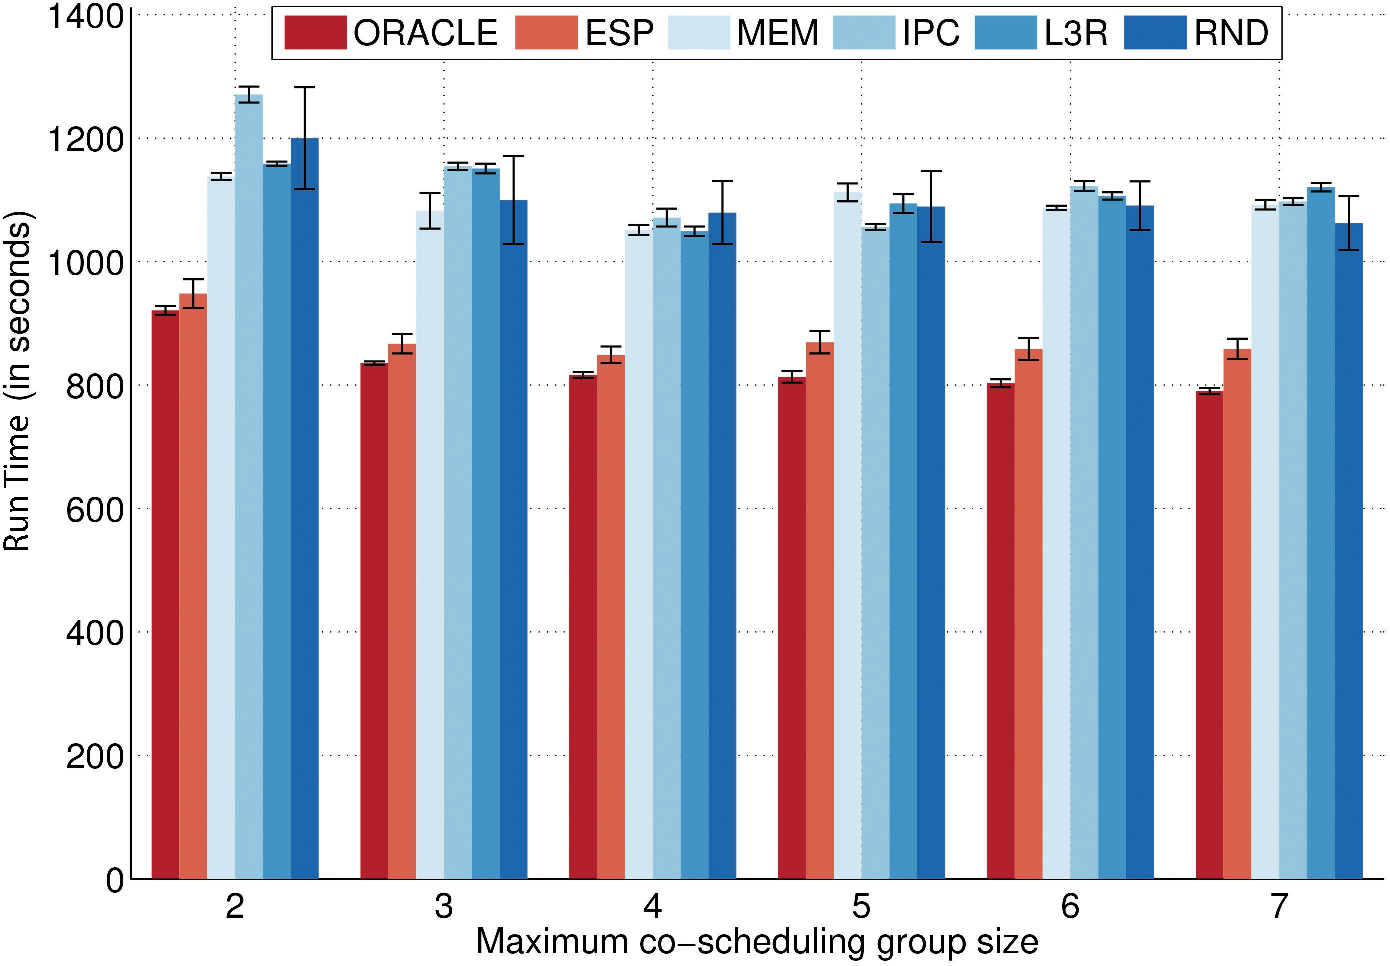
\includegraphics[width=0.7\textwidth]{figures/barmainCOPY.pdf}
 \caption{\small Single processor scheduling performance. On an
   average over different $k$, \SYSTEM{} is 25\% better than MEM, 29\%
   better than IPC, 27\% better than L3R, 26\% better than RND, and
   only 5\% worse than ORACLE. }
\label{fig:bar_single_processor}
\end{center}
\end{figure}

\begin{figure*}[t]
  \begin{center}
    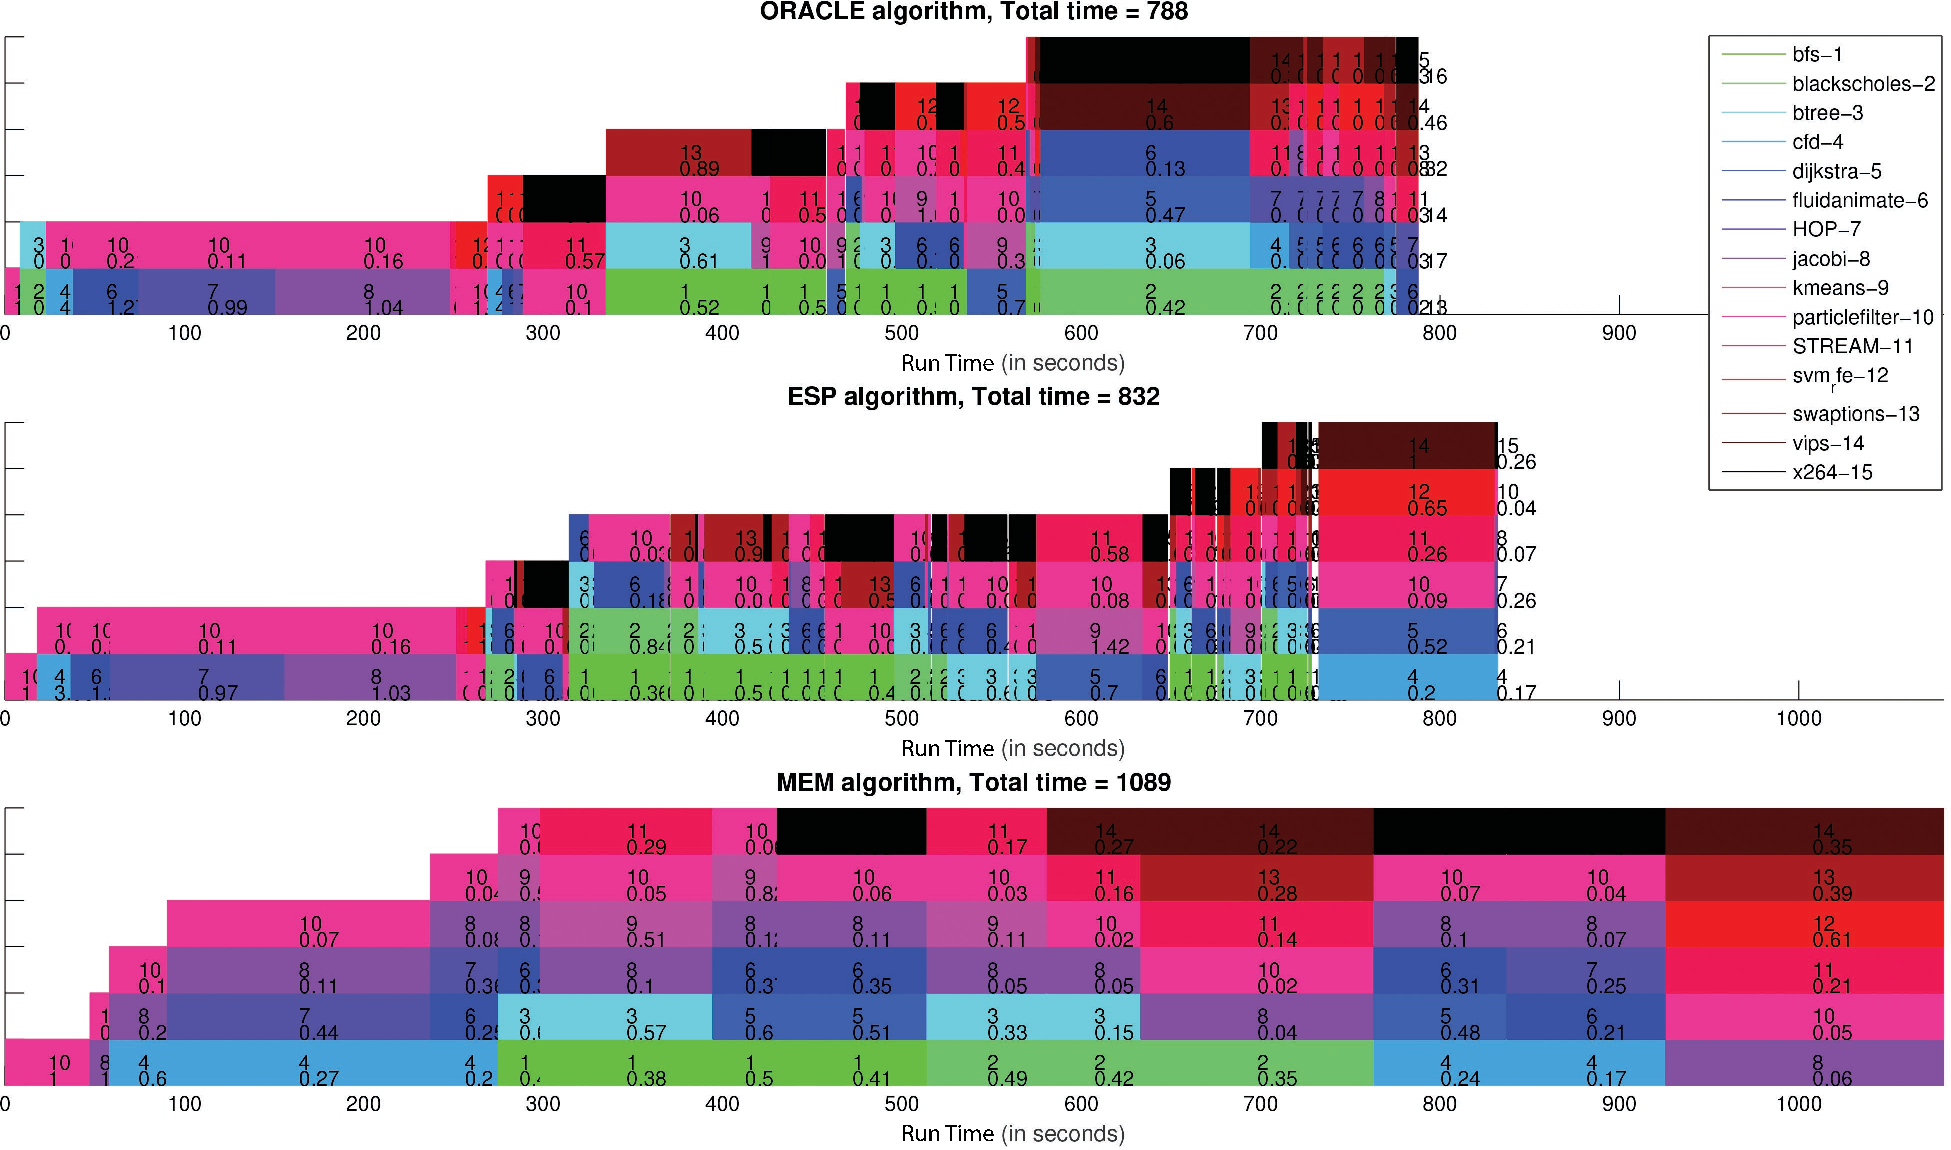
\includegraphics[width=1\textwidth]{figures/scheduleCOPY.pdf}
    \caption{\small Comparison of schedules obtained from different
      algorithms with up-to 6 co-scheduled applications ($k$ = 6) (more
      compact is better). Each block represents an application running
      with other applications. The number in the top of the block
      represents the application index. The number at the bottom
      represents the slowdown the application experiences.  The
      schedule built using \SYSTEM{} algorithm squeezes the
      applications together better than the MEM baseline.}
    \label{fig:schedule2}
  \end{center}
\end{figure*}
\begin{figure*}[t]
\begin{center}
 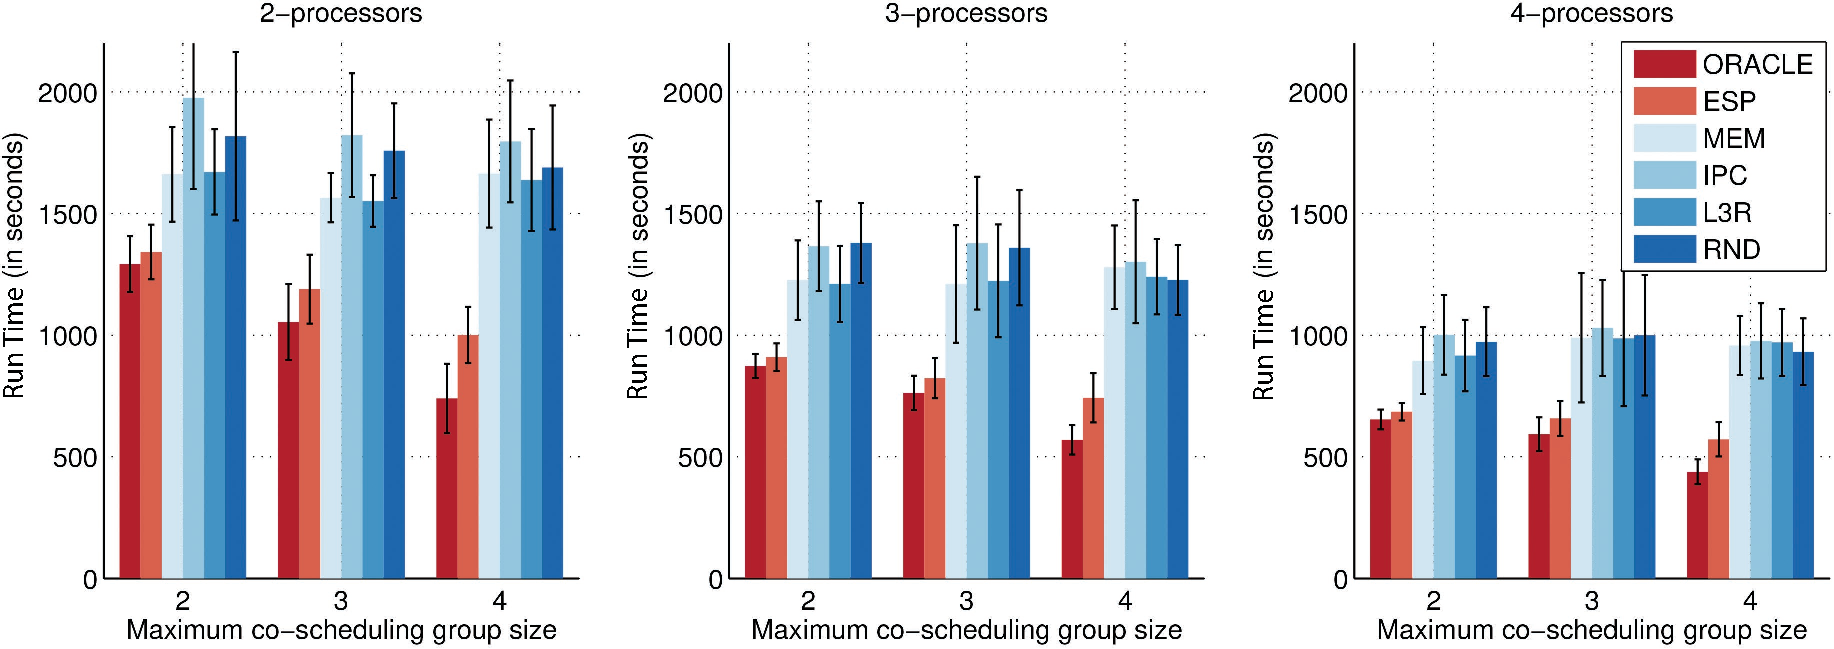
\includegraphics[width=1\textwidth]{figures/parallel_schedule_combb_all_mayCOPY.pdf}
 \caption{\small Comparison of multi-node scheduling times for stream
   of 40 applications (lower is better). On an average over different
   processes and tuples, \SYSTEM{} is 47\% better than MEM, 61\%
   better than IPC, 47\% better than L3R and 54\% better than RND. }
\label{fig:expt:multi-node-all}
\end{center}
\end{figure*}

\begin{figure*}[!t]
\begin{center}
 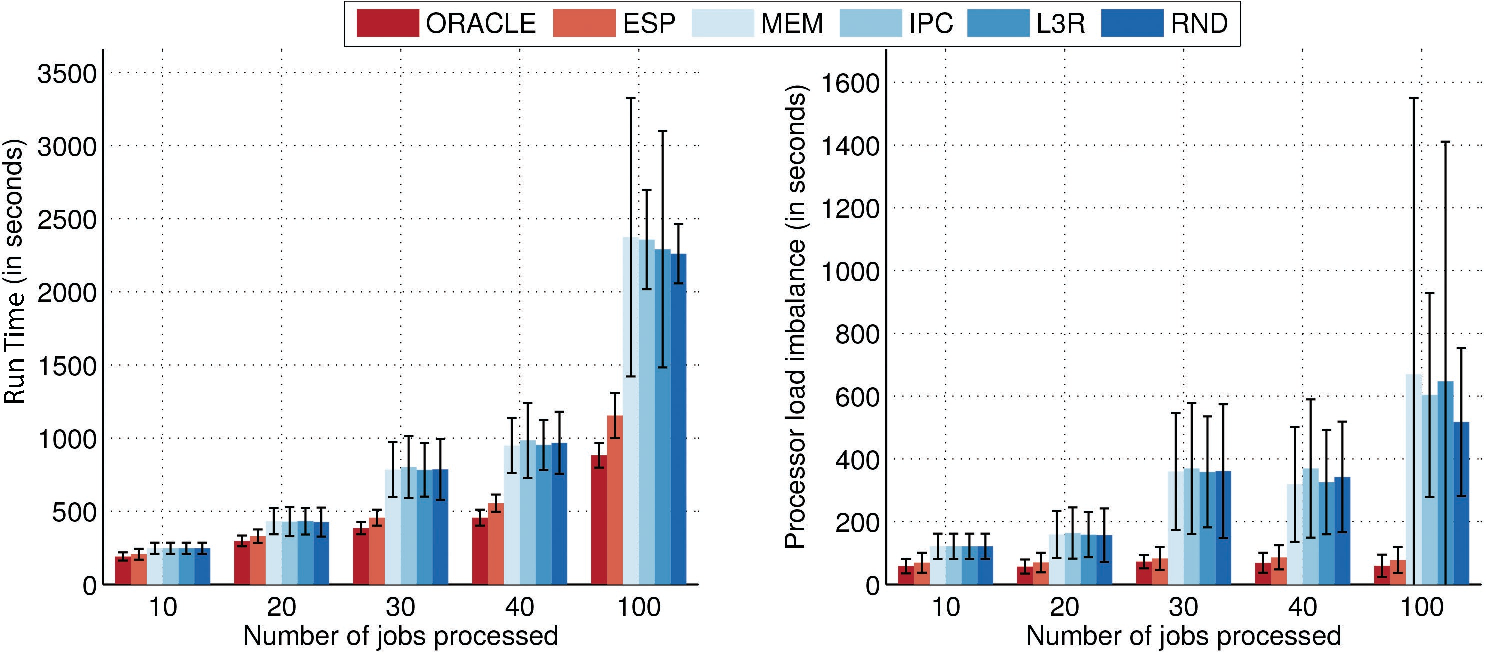
\includegraphics[width=0.9\textwidth]{figures/parallel_schedule_combb_100jobs_load_4_4_load_imbalance_combinedCOPY.pdf}
 \caption{\small Multi-node scheduling performance with varying number
   of incoming jobs, allowing up to 4 co-scheduled applications per
   node (lower is better). The left figure shows scheduling time (in
   seconds) -- on average \SYSTEM{} is 60\% better than MEM, 61\%
   better than IPC, 58\% better than L3R and 58\% better than RND. The
   right figure shows the load imbalance (the difference between the
   highest and lowest scheduling time across nodes).  As we increase
   the number of jobs the load imbalance increases faster for the
   baseline algorithms and seems relatively constant for \SYSTEM{} and
   the ORACLE.}
\label{fig:expt:multi-node-100}
\end{center}
\end{figure*}

\subsection{Single Node Scheduling Results}
\label{sec:sched_single_proc}
To test single-node batch scheduling, we launch all 15 benchmarks
listed in \secref{setup}.  The schedulers order application execution
to minimize total job completion time.  We vary $k$, the maximum
number of applications that can be co-scheduled from two to six.  We
find that it is never beneficial to schedule more than six
applications simultaneously and no scheduler (other than random) ever
attempted to do so even when more were allowed.  We run 15 separate
experiments for each $k$, where each experiment differs by the split
between training and testing data for \SYSTEM{}.


\figref{fig:bar_single_processor} shows the results. The x-axis is
$k$, the y-axis is the time to complete the work, and there is a bar
showing the mean scheduling time for each of our points of comparison
with an error bar showing one standard deviation.
% During the offline phase, we first sample a few configurations
% followed by calculating the estimated performance those samples;
% overhead of which is discussed in the next section(Section
% \secref{expt:overhead}). Once we do the estimation of the performance
% using \SYSTEM{} individually for each $k = 2:6$ ($k$ denotes the
% maximum number of applications we are willing to co-schedule
% together), we run Algorithm \ref{alg:ItrSched-multi} to schedule those
% applications. We notice that, as per our intuition, as we allow more
% applications to run together, the scheduling time for the ORACLE
% decreases. But, the scheduling time does not decrease significantly
% after 4-tuples. On the other hand for \SYSTEM{} the scheduling time
% decrease until 4-tuples and slightly increases after that. We
% attribute this to the fact that as we estimate more tuples the overall
% estimation error is piling up and since the benefit of running more
% applications together dwindles after 4-tuples, the extra noise in the
% system makes approximate scheduling using \SYSTEM{} slightly worse. We
% see similar behavior for scheduling even in the baseline algorithms,
% where we see improvement only up-to a certain point.
Overall, \SYSTEM{} performs much better than the baseline algorithms
and only slightly worse than the ORACLE. On average over different
$k$, \SYSTEM{} is 25\% faster than MEM, 29\% faster than IPC, 27\%
faster than L3R and 26\% faster than RND.  These results include
prediction and scheduling overhead, yet \SYSTEM{} is only 5\% worse
than the ORACLE, which has no overhead and knows the future.  We
conclude that \SYSTEM{} produces highly accurate predictions and yet
is efficient enough for practical use.


To provide intuition on the different schedulers,
\figref{fig:schedule2} illustrates the schedules produced by: ORACLE
(top), \SYSTEM{} (middle), and MEM (bottom) when they are allowed to
co-schedule up to six applications.  For each chart, the horizontal
axis represents time in seconds. Each colored block represents an
application running with other applications. The top number in the
block represents the application index (see the legend for mapping
from index to name), and the bottom number represents the actual
slowdown the application experienced at that time (this actual
slowdown is determined after the fact).  A better schedule is more
compact and completes further to the left.  Clearly, \SYSTEM{}'s
schedule is more compact and closer to the ORACLE than MEM.  ORACLE
runs the maximum number of applications together less than half of the
time.  MEM, in contrast, runs the maximum allowed number of
applications most of the time. Overall in this particular instance,
the scheduling time for the ORACLE is 788 seconds, 832 for \SYSTEM{},
and 1089 for MEM.




\subsection{Multi-node Scheduling Results}
\label{sec:sched-multi-node}
In this section we discuss multi-node scheduling performance. We use
two, three, and four copies of our base test platform (described
above).  We assume that applications arrive randomly from our set of
15 benchmarks (so some benchmarks may have multiple instances live in
the system).  The challenge is to assign an application to a
processor as it arrives such that the total impact on the system is
minimized; \ie put the application on the node that minimizes
interference.

The oracle computes the best possible schedule, the heuristics use
activity vectors to select the best node and the \SYSTEM{}-based
approach uses Algorithm \ref{alg:ItrSched-multi}.
\figref{fig:expt:multi-node-all} summarizes the results for 2, 3 and 4
processors and for $k = 2,3$ or $4$. As we increase the number of
processors, the scheduling time improves for all approaches. \SYSTEM{}
performs almost as well as the ORACLE, performing 5\% to 13\% worse on
an average.  In fact, \SYSTEM{} is always within 1 standard deviation
of ORACLE. \SYSTEM{} performs significantly better than the activity
vector algorithms. On average over different processes and tuples,
\SYSTEM{} is 47\% better than MEM, 61\% better than IPC, 47\% better
than L3R, and 54\% better than RND.  Additionally, the standard
deviation in performance for \SYSTEM{} is much lower compared to the
baseline algorithm, leading to much better performance predictability.
This predictability is further evidence of our claim that \SYSTEM{}
allows the schedulers to avoid bad predictions.

\subsection{Multi-node Sensitivity to Job Size}
\label{sec:exp:multi-node-job}
We also study the scheduling performance as a function of the total
number of applications scheduled. To be clear, jobs are still
scheduled as they arrive (the multi-node scheduler does not reorder
applications), we simply have more of them.  Specifically, we send up
to 100 jobs to a system with 4 nodes and we are allowed to co-schedule
up to 4 applications together.  For each experiment, we perform 15
trials with different random job arrivals.  All results report the
mean with error bars indicating one standard deviation.

\figref{fig:expt:multi-node-100} shows how scheduling performance
changes as a function of the total number of applications scheduled.
The figure consists of two charts: the one on the left showing
scheduling time as a function of applications scheduled and the one on
the right showing load imbalance in terms of the largest difference in
execution time between one processor and another. The number of
applications scheduled is shown on the x-axis and the time on the
y-axis.  As the number of applications increases, \SYSTEM{}'s relative
performance improves compared to the activity vector approaches. The
key to this result is \SYSTEM{}'s accurate quantification of
interference.  The ability to directly reason about slowdown allows
the \SYSTEM{}-based approach to rank scheduling decisions and always
choose the one with the least impact on the performance of both the
running applications and the application that just arrived.

\SYSTEM{}'s foresight becomes more crucial as the number of jobs
increase because bad decisions can create severe load imbalance on the
parallel machine, as shown on the right side of
\figref{fig:expt:multi-node-100}. As we increase the number of jobs
the processor load imbalance increases vastly for the activity vector
approaches and seems relatively constant for \SYSTEM{} as well as
ORACLE. On an average \SYSTEM{} is 60\% better than MEM, 61\% better
than IPC, 58\% better than L3R and 58\% better than RND. Again, the
standard deviation (shown by the error bars) for \SYSTEM{} is much
lower than the baselines---leading to much more predictable
performance for latency sensitive applications.


\begin{figure*}[t]
\begin{center}
 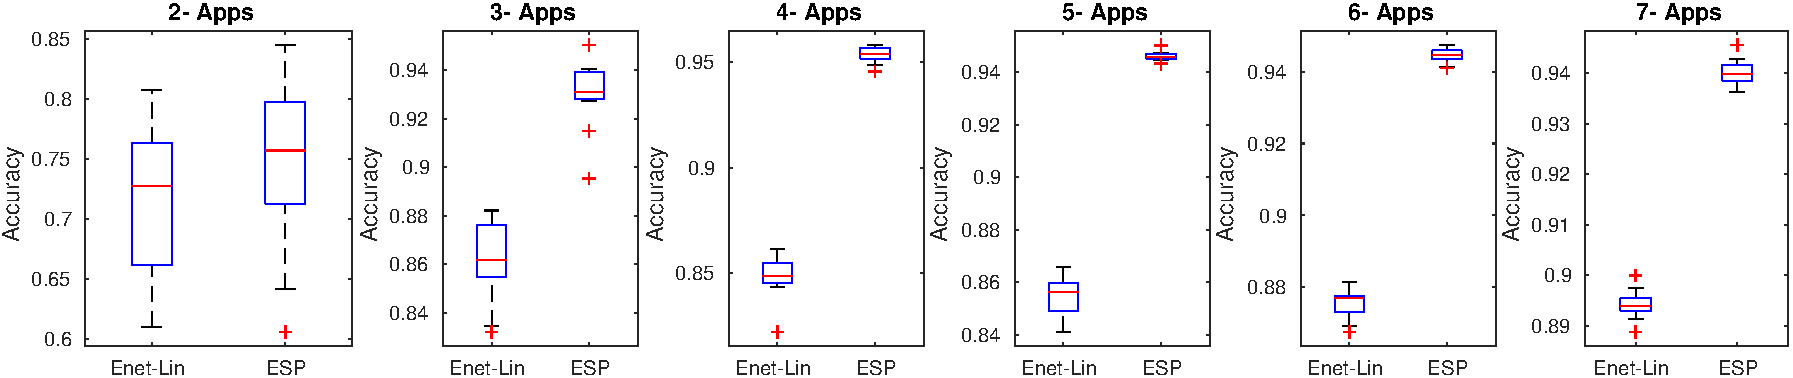
\includegraphics[width=1\textwidth]{figures/accuracy_boxplot_ridge_lasso_enet2.pdf}
 \caption{\small Prediction accuracy comparison between Enet-lin and
     \SYSTEM{}.
     % We use 70\% of the data during training phase and
     %  predict the remaining 30\% of the samples.
   }
\label{fig:est:box-plot}
\end{center}
\end{figure*}
\PUNT{
\begin{table*}[t]
\centering
\caption{Overhead}
\footnotesize
\begin{tabular}{ c|c|c|c|c|c|c|c }
 \hline
 \hline
 &k & 2 & 3 &4 & 5 & 6 & 7 \\
 \hline
\multirow {3}{*}{\SYSTEM{}}  & Model training (in seconds)   & 0.42    & 0.59 &   0.68 & 0.69 & 0.48 & 0.51\\
& Prediction time (in seconds)  &   0.00056  & 0.003   &0.0076 & 0.0198 & 0.04 & 0.06\\
& Training sample size (in \%)  & 70\% & 40 \% &  10 \% & 4\% & 1 \% & 1\% \\ \hline \hline
\multirow {2}{*}{Scheduling Algorithm \ref{alg:ItrSched}}  & \SYSTEM{} (in seconds)    &0.52 & 1.18&  2.08 & 3.17 & 4.19 & 5.57\\
& Linear program (in seconds) &   0.12 & 0.21 & 0.35 & 0.9 & 1.75 & 3.3 \\
 \hline
 \hline
\end{tabular}
 \label{table:overhead}
\end{table*}
}

\begin{table*}[t]
\centering
\caption{Overhead}
\footnotesize
\begin{tabular}{ c|c|c|c|c|c|c|c }
 \hline
 \hline
 &k & 2 & 3 &4 & 5 & 6 & 7 \\
 \hline
\multirow {3}{*}{\SYSTEM{}}  & Model training (in seconds)   & 0.42    & 0.59 &   0.68 & 0.69 & 0.48 & 0.51\\
& Prediction time (in seconds)  &   0.00056  & 0.003   &0.0076 & 0.0198 & 0.04 & 0.06\\
& Training sample size (in \%)  & 70\% & 40 \% &  10 \% & 4\% & 1 \% & 1\% \\ \hline \hline
\multirow {1}{*}{Scheduling Algorithm \ref{alg:ItrSched}}  & Linear program (in seconds/job) &   0.008 & 0.014 & 0.023 & 0.06 & 0.117 & 0.22\\
 \hline
 \hline
\end{tabular}
 \label{table:overhead}
\end{table*}

\subsection{\SYSTEM{} Prediction Accuracy}
\label{sec:st_model}
%The preceding sections show the benefits of integrating \SYSTEM{} into
%single and multi-node schedulers.  We assert that \SYSTEM{}'s accurate
%quantifiable predictions are the key to its success.  Here we analyze
%that accuracy directly.

We compare \SYSTEM{} with the \textit{elastic-net} regularization
method on the linear model (\textit{Enet-lin}) described in
\secref{est:elastic-net}.  \PUNT{The comparisons are based on
  prediction accuracy for both the models.  vs sample complexity,
  specifically how many samples are required to reach 90\% accuracy.
  Throughout this section, we refer to one sample as a measurement of
  a group of $k$-applications which generates $k$ readings
  corresponding to each of the applications in the group.} To evaluate
quantitatively, we measure the \emph{accuracy} of the predicted
performance $\hat{\z}$ with respect to the true data $\z$, by
computing the \emph{coefficient of determination} ($R^2$ value):
\begin{equation}
\label{eq:accuracy}
\text{accuracy}(\hat{\z},\z) = \left(1 - \frac{\| \hat{\w}-\w \|^2_2}{\| \w - \bar{\w}\|^2_2}\right)_{+},
\end{equation}
where $\w = \min(\z,\boldsymbol{1})$ and $\hat{\w} =
\min(\hat{\z},\boldsymbol{1}).$ This metric captures how well the
predicted results correlate with the measured results. Unity
represents perfect correlation.



%\subsubsection{Prediction accuracy}
\figref{fig:est:box-plot} shows a box-plot for out-of-sample
predictive accuracy of \SYSTEM{} and Enet-lin when we train both the
models with 70\% data and test the prediction on the remaining data.
For $k=2$, \SYSTEM{} performs only slightly better than the Enet-lin
with on average 76\% accuracy whereas the baseline is 73\% accurate.
For $k>2$, the prediction accuracy for the \SYSTEM{} varies from 93\%
to 96\% with very small variance. On the other hand, Enet-lin is only
between 85\% to 88\% accurate.

% \begin{figure*}[!htbp]
% \begin{center}
%  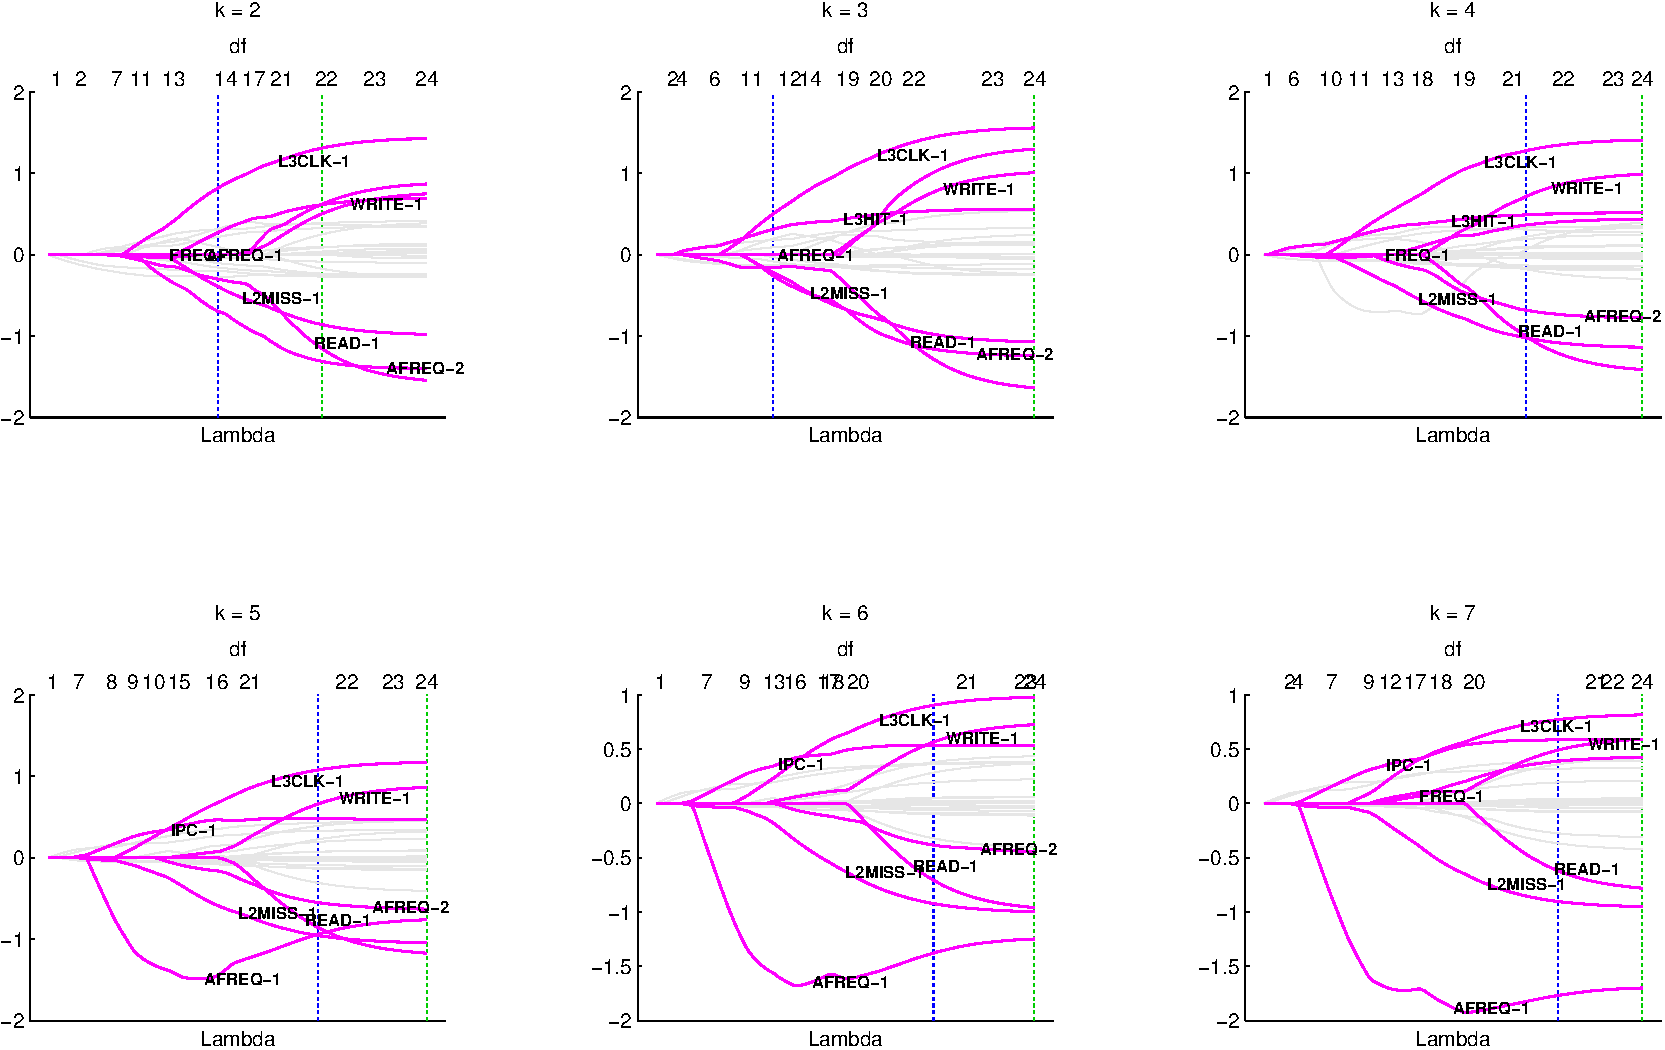
\includegraphics[width=1\textwidth]{figures/solution_path_general.pdf}
%  \caption{ A solution path diagram using elastic-net for a linear model (no interaction terms) with just an important subset of variables so that it is easier to visualize.  Each dark solid line in the plot represents a variable's coefficient. The corresponding variable is mentioned on the line. The dashed blue line indicates largest $\lambda$ such that MSE is within one standard error of the minimum, a scalar and the dashed green line corresponds $\lambda$ value with minimum MSE.  Since, the variables in the design matrix are highly correlated, variable signs may not be correctly represented.}
% \label{fig:est:solution-path}
% \end{center}
% \end{figure*}
% \subsubsection{Discussion for the solution path for regression models}
% We wanted to build some more intuition about the variable selection
% and how the model evolves over different values for $k$. In
% \figref{fig:est:solution-path}, we show a variable in and out plot and
% what is known as a \textit{solution path} in statistics. The x-axis is
% the regularization parameter $\lambda$ and y-axis is the coefficient
% size. For the co-efficient size to relatively make sense we have
% normalized the columns of the design matrix to have Euclidean-norm
% equal to 1. As we increase $\lambda$ the regularization becomes less
% strict and more and more variables can enter the model. In this figure
% we have a solution path diagram using elastic-net for a linear model
% (no interaction terms) with just an important subset of variables so
% that it is easier to visualize.  Each dark solid line in the plot
% represents a variable's coefficient and how it changes as we increase
% lambda.  The corresponding variable is mentioned on the solid plot
% line itself. The dashed blue line indicates largest $\lambda$ such
% that MSE is within one standard error of the minimum, a scalar and the
% dashed green line corresponds $\lambda$ value with minimum MSE.
% Since, the variables in the design matrix are highly correlated, a
% positive (or a negative) variable in this diagram does not mean that
% it certainly positively (or negatively) affects the performance. But,
% if the variable has large absolute value, we can still claim that,
% conditioned on other variables selected in the model it has large
% impact. What is interesting in this figure is how as $k$ increases the
% model evolves. $k=2, 3$ and $4$ have similar solution paths and $k=5,
% 6$ and $7$ has similar path but the two paths are a bit different from
% each other, indicating some phase transition happening at $k=4$. This
% indicates that there might be an opportunity to predict performance
% for larger $k$'s by aggregating data for smaller $k$. This can be very
% important for datacenters where they only observe very large number of
% applications co-scheduled together.



\subsection{Overhead}
\label{sec:expt:overhead}
\SYSTEM{} has an offline sampling phase followed by an
estimation phase. Once we have collected the samples from the batch of
co-scheduled applications, we run \SYSTEM{} to obtain the predictions
for the rest of the combinations of the applications. We have
summarized the overhead results in the Table \ref{table:overhead}. We
require less than 0.7 seconds to build the performance model for a
batch of $k$-tuples running together. Once the model is built, the
prediction time for \SYSTEM{} is very small and would range from 0.5
milliseconds to 60 milliseconds. For such small training data, the
prediction accuracy for $k=2$ is around $80\%$ and for $k>2$ it is
around $86\%$.

The scheduling overhead, again has two components: first obtaining the
application's batch run profile which is done using \SYSTEM{}, and
then solving the linear program to obtain the schedule. The first part
(in the top of Table \ref{table:overhead}) is done offline.  The vast
bulk of online work is done by Equation \eqref{eq:schedule_general2},
which solves a very sparse optimization problem. The total overhead
per scheduled job for Algorithm \ref{alg:ItrSched} -- the online
portion of the approach -- ranges from 0.008 seconds for $k=2$ to 0.22
seconds for $k=7$. Almost all of this work could be parallelized on a
multicore (or accelerated with SIMD instructions) but that is beyond
the scope of this work.  We note that it is quite practical to
consider co-scheduling up to 4 jobs.  The overhead of scheduling $7$
jobs may become prohibitive, but it is never useful on our test
system.  This is not an insignificant amount of time but this approach
is suitable for long running applications and the benchmarks that we
have used in this paper are all long running benchmarks with at least
10 seconds of individual runtime.
